\documentclass[]{report}

\usepackage[utf8]{inputenc}
\usepackage[spanish]{babel}
\usepackage{graphicx}
\graphicspath{{imagenes/}}
\usepackage[colorlinks]{hyperref}
\usepackage[svgnames]{xcolor}
\hypersetup{citecolor=DarkRed}
\hypersetup{linkcolor=DarkBlue}
\hypersetup{urlcolor=DarkBlue}

% Title Page
\title{Agrupamiento difuso}
\author{Carlos Cobos Suárez\\Adrián Morente Gabaldón}


\begin{document}
\maketitle

\begin{abstract}
	
	Este trabajo consiste en exponer las limitaciones del agrupamiento o \textit{clustering} clásico para resolverlas tras estudiar cómo la lógica difusa puede ayudar en la modelización del problema. 
	
	Se darán a conocer los tipos de modelos de agrupamiento usando lógica difusa, así como sus características y limitaciones intentando resolverlas con otro tipo de modelo.
	
	Para terminar y entender que los modelos expuestos tienen una gran relevancia en nuestra sociedad, se citarán aplicaciones reales que hacen uso de estos modelos.
	
\end{abstract}

	\chapter{Agrupamiento clásico}
	
		\section{Definición}
		
			Entendemos por \textbf{agrupamiento clásico} a la técnica de clasificación de datos en distintas categorías según su similitud (o \textit{distancia}, si los entendemos como una representación de puntos en un espacio determinado).
			
			\begin{figure}[h]
				\centering
				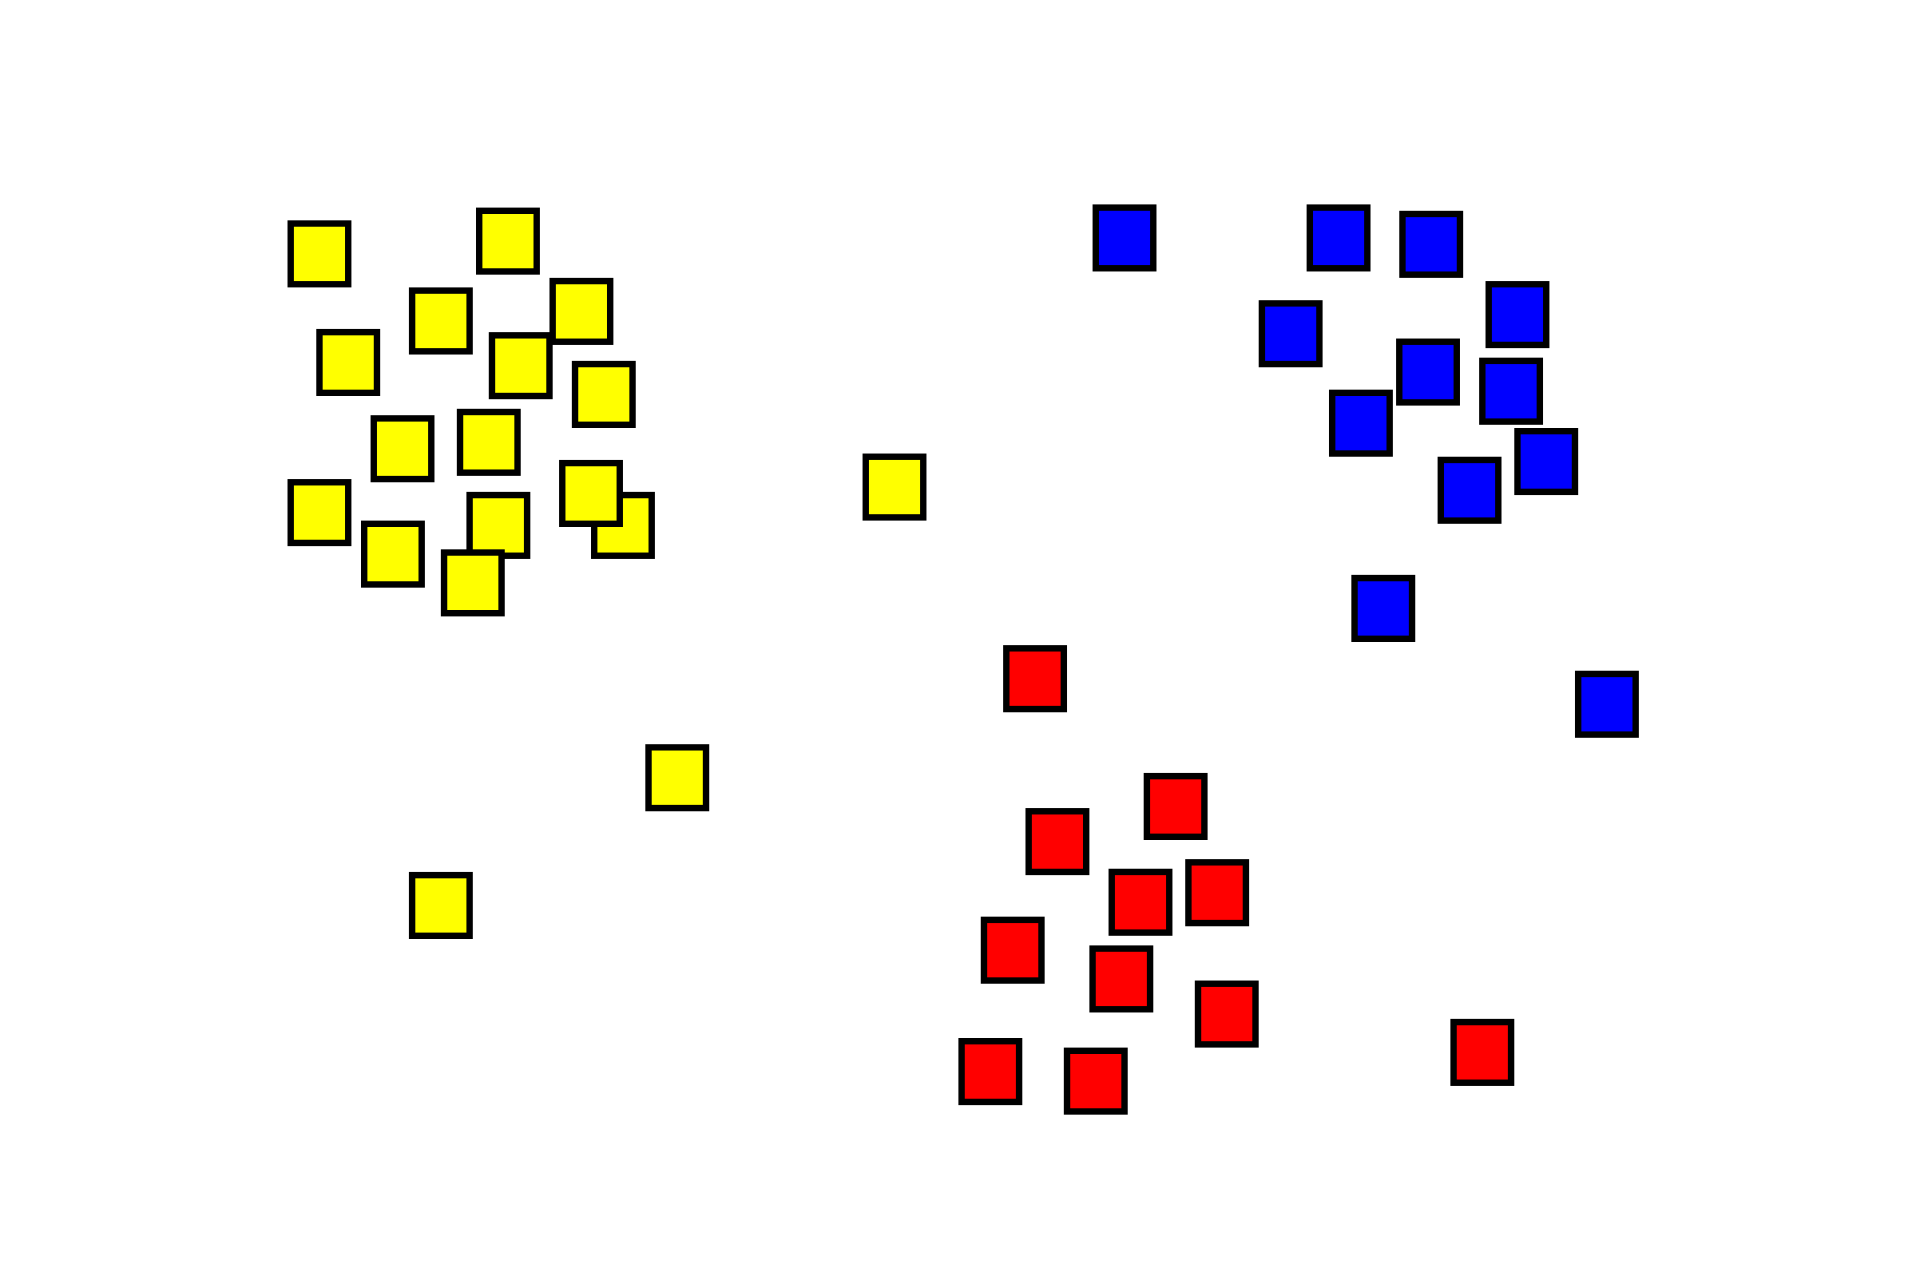
\includegraphics[width=0.5\textwidth]{clustering.png}
				\label{clustering1}
				\caption{Ilustración de agrupamiento clásico. \href{https://en.wikipedia.org/wiki/Cluster_analysis\#/media/File:Cluster-2.svg}{ \textit{(Wikimedia Creative Commons)}}}
			\end{figure}
		
			Se trata de una tarea principal en la labor de minería de datos a modo exploratorio, además de una técnica común para análisis estadístico de datos (aprendizaje automático, reconocimiento de patrones, análisis de imágenes, etc.).
					
		\section{Conceptos}
		
			Para entender con mayor profundidad los fundamentos del \textit{clustering}, deben interiorizarse algunos conceptos clave:
			
			\begin{itemize}
				\item \textbf{Clúster \textit{(o cluster)}}: se trata de cada una de las categorías o grupos en los que se clasifican finalmente los datos. Esto es, según vemos en la figura \ref{clustering1}, los distintos colores que identifican a cada grupo.
				\item \textbf{Centroide}: se conoce como tal al punto de referencia de cada \textit{cluster}. Puede ser el objeto más característico de los clasificados en un grupo (por ejemplo, si estamos clasificando datos en colores y encontramos un grupo \textbf{amarillo}, el centroide se correspondería con el dato \textit{más amarillo} de todos ellos (realizaremos apuntes sobre esto más adelante).
				\item \textbf{Función de distancia}: 
			\end{itemize}
		
		\section{Limitaciones}
	
	\chapter{Agrupamiento difuso}
		Tal y como se acaba de ver, el agrupamiento clásico tiene una limitación bastante importante y es la de que un sólo dato puede pertenecer a un \textit{cluster}. Esto también tiene la consecuencia de que, dependiendo del algoritmo de agrupamiento que se vaya a emplear, no se puede garantizar la convergencia del mismo.
		
		A demás, si se usan redes neuronales para llevar a cabo la labor de agrupar los datos, es natural y lógico pensar que un sólo dato va a provocar la activación de más de una neurona. Es por ello que se tiene que cambiar el modelo clásico a uno más permisivo en el cual se solucionen dichos problemas.
			
		\section{Definición}
			
		
		\section{Limitaciones}
	
	\chapter{Agrupamiento difuso posibilístico}
	
		\section{Definición}
	
	\chapter{Aplicaciones reales}
	
\bibliographystyle{plain}
\bibliography{citas}

\end{document}          
